\author{Miggiano Davide 4840761\\ Morando Andrea 4604844}
\date{}
% Options for packages loaded elsewhere
\PassOptionsToPackage{unicode}{hyperref}
\PassOptionsToPackage{hyphens}{url}
%
\documentclass[12pt,a4paper]{article}
\usepackage{amsmath,amssymb}
\usepackage{lmodern}
\usepackage{iftex}
\usepackage{placeins}
\usepackage{graphicx}
\usepackage{tabularx}
\usepackage[left=2.5cm,right=2.5cm,top=1.5cm,bottom=1.5cm]{geometry}

\ifPDFTeX
  \usepackage[T1]{fontenc}
  \usepackage[utf8]{inputenc}
  \usepackage{textcomp} % provide euro and other symbols
\else % if luatex or xetex
  \usepackage{unicode-math}
  \defaultfontfeatures{Scale=MatchLowercase}
  \defaultfontfeatures[\rmfamily]{Ligatures=TeX,Scale=1}
\fi
% Use upquote if available, for straight quotes in verbatim environments
\IfFileExists{upquote.sty}{\usepackage{upquote}}{}
\IfFileExists{microtype.sty}{% use microtype if available
  \usepackage[]{microtype}
  \UseMicrotypeSet[protrusion]{basicmath} % disable protrusion for tt fonts
}{}
\makeatletter
\@ifundefined{KOMAClassName}{% if non-KOMA class
  \IfFileExists{parskip.sty}{%
    \usepackage{parskip}
  }{% else
    \setlength{\parindent}{0pt}
    \setlength{\parskip}{6pt plus 2pt minus 1pt}}
}{% if KOMA class
  \KOMAoptions{parskip=half}}
\makeatother

\usepackage{xcolor}
\usepackage{graphicx}
\usepackage{listings}

\makeatletter
\def\maxwidth{\ifdim\Gin@nat@width>\linewidth\linewidth\else\Gin@nat@width\fi}
\def\maxheight{\ifdim\Gin@nat@height>\textheight\textheight\else\Gin@nat@height\fi}
\makeatother
% Scale images if necessary, so that they will not overflow the page
% margins by default, and it is still possible to overwrite the defaults
% using explicit options in \includegraphics[width, height, ...]{}
\setkeys{Gin}{width=\maxwidth,height=\maxheight,keepaspectratio}
% Set default figure placement to htbp
\makeatletter
\def\fps@figure{htbp}
\makeatother
\setlength{\emergencystretch}{3em} % prevent overfull lines
\providecommand{\tightlist}{%
  \setlength{\itemsep}{0pt}\setlength{\parskip}{0pt}}
\setcounter{secnumdepth}{-\maxdimen} % remove section numbering
\ifLuaTeX
  \usepackage{selnolig}  % disable illegal ligatures
\fi
\IfFileExists{bookmark.sty}{\usepackage{bookmark}}{\usepackage{hyperref}}
\IfFileExists{xurl.sty}{\usepackage{xurl}}{} % add URL line breaks if available
\urlstyle{same} % disable monospaced font for URLs
\hypersetup{
  hidelinks,
  pdfcreator={LaTeX via pandoc}}

% Define JSON styling
\lstdefinelanguage{json}{
    basicstyle=\ttfamily\small,
    numbers=left,
    numberstyle=\tiny\color{gray},
    stepnumber=1,
    numbersep=8pt,
    showstringspaces=false,
    breaklines=true,
    frame=single,
    backgroundcolor=\color{white},
    stringstyle=\color{orange},
    keywordstyle=\color{blue}\bfseries,
    morekeywords={true,false,null}
}
\begin{document}

\title{Crime Monitoring and Analysis in Los Angeles.}
\maketitle

\section{Proposed Domain and Application}
The Application we propose is the Crime Trend Analysis and Prediction System for Los Angeles Police Department (LAPD). The system provides:
\begin{itemize}
    \item Real-time crime reporting visualization on an interactive map.
    \item Prediction of crime trends by analyzing temporal and spatial crime patterns.
    \item Neighborhood safety scoring based on historical and current crime data.
    \item Identifying safer streets in the city.
    \item Social analysis of crime, including demographic information to help law enforcement understand crime behaviors.
\end{itemize}

\subsection{Application details}
Main characteristics:
\begin{itemize}
    \item \textbf{Read/Write Nature}: The application is read-intensive, with frequent analytical queries from law enforcement and local authorities. It also has periodic batch write operations as new crime reports are processed and stored, on average with around 650 crimes each day.
    \item \textbf{System Requirements}: 
    \begin{itemize}
        \item \textbf{Consistency}: Strong consistency is required for certain operations (e.g., ensuring accurate crime count by location), but eventual consistency might be acceptable for non-critical operations like trend prediction.
        \item \textbf{High Availability}: High availability is critical to ensure that the system remains accessible for real-time monitoring.
    \end{itemize}
\end{itemize}

\newpage
\section{Conceptual Schema}
\begin{figure}
    \centering
    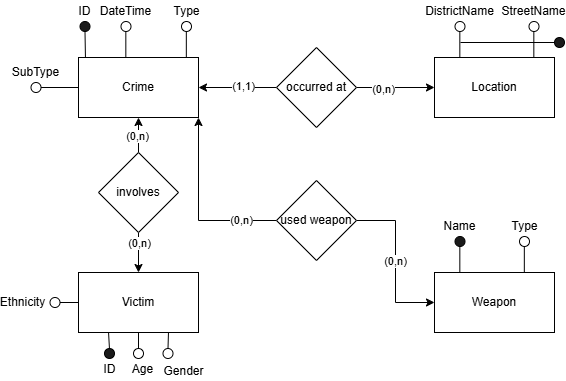
\includegraphics[width=0.8\linewidth]{adm.drawio.png}
    \caption{ER Schema}
    \label{fig:enter-label}
\end{figure}

\section{Workload}
\begin{enumerate}
    \item Find all crimes and their type that occurred in a given district and in a given time interval;
    \item Identify all victims given a crime type;
    \item Count all crimes involving a certain type of weapon;
    \item Find the crimes and victims of a given district;
    \item Given an ethnicity find all streets in which that ethnicity has experienced crimes, sorting them by the number of crimes.
\end{enumerate}

\newpage
\section{Aggregate-oriented Design Methodology}
\[
\begin{aligned}
Q1: & \quad (\text{Crime}, \; [\text{Crime(DateTime)} \, \_!, \; \text{Location(DistrictName)} \, \_OA], \; [\text{Crime(ID, Type)} \, \_!]) \\
Q2: & \quad (\text{Crime}, \; [\text{Crime(Type)} \, \_!], \; [\text{Victim(Age, Gender, Ethnicity)} \, \_I]) \\
Q3: & \quad (\text{Weapon}, \; [\text{Weapon(Type)} \, \_!], \; [\text{Crime(ID)} \, \_UW]) \\
Q4: & \quad (\text{Location}, \; [\text{Location(DistrictName)} \, \_!], \; [\text{Crime \_OA}, \; \text{Victim\_IOA}]) \\
Q5: & \quad (\text{Victim}, \; [\text{Victim(Ethnicity)} \, \_!], \; [\text{Location(StreetName)} \, \_OAI, \; \text{Crime(ID)} \, \_I])
\end{aligned}
\]

\begin{figure}
    \centering
    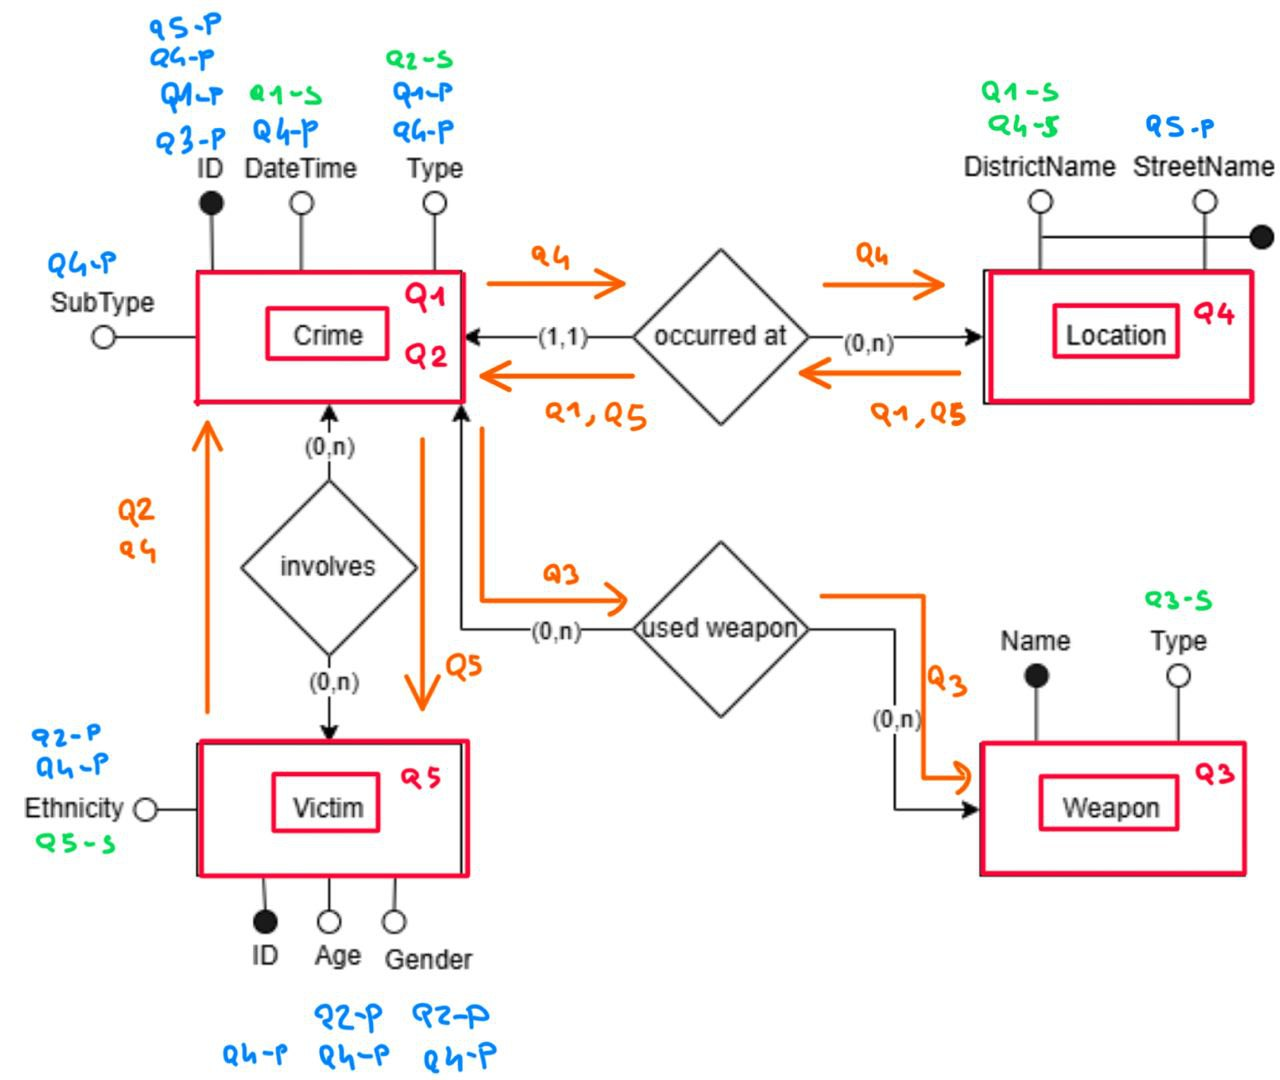
\includegraphics[width=0.8\linewidth]{annotated_schema.jpg}
    \caption{Annotated ER Schema}
    \label{fig:enter-label}
\end{figure}

\begin{itemize}
    \item \textbf{\textit{crime}}: {\underline{Id}, DateTime, DistrictName, Victims: [{Ethnicity, Age, Gender}]}
    \item \textbf{\textit{weapon}} : {\underline{Name}, Type, CrimeIds : [...]}
    \item \textbf{\textit{location}} : {\underline{DistrictName}, Crimes : [{Id, DateTime, Type, Subtype}], Victims : [{Id, Age, Gender, Ethnicity}]}
    \item \textbf{\textit{victim}} : {\underline{Id}, Ethnicity, CrimeId, StreetName}
\end{itemize}

\section{Design in MongoDB}
\section{Design in Cassandra}
\section{Design in Neo4J}
\section{Most Suitable System among the designed ones}


\end{document}1